\documentclass[aspectratio=169]{beamer}

\usetheme{Boadilla}
\usefonttheme{professionalfonts}
\setbeamertemplate{navigation symbols}{}
\setbeamertemplate{itemize items}[circle]
\setbeamertemplate{enumerate items}[default]
\setbeamertemplate{headline}{}

\usepackage[utf8]{inputenc}
\usepackage[T1]{fontenc}
\usepackage{lmodern}
\usepackage{amsmath}
\usepackage{booktabs}
\usepackage{tabularx}
\usepackage{array}
\usepackage{hyperref}
\usepackage[strings]{underscore}
\usepackage{listings}
\usepackage{tikz}
\usetikzlibrary{arrows.meta,positioning,fit,calc,shapes.geometric}
\usepackage{xcolor}

\definecolor{courseblue}{HTML}{12355B}
\definecolor{coursegold}{HTML}{C98A2E}
\definecolor{courseice}{HTML}{EEF3F8}
\definecolor{coursegreen}{HTML}{2F6B4F}
\definecolor{coursegray}{HTML}{4B5563}
\definecolor{codebg}{HTML}{F7F9FC}
\definecolor{codecomment}{HTML}{5E6C84}
\definecolor{codestring}{HTML}{0B6E4F}

\setbeamercolor{palette primary}{bg=courseblue,fg=white}
\setbeamercolor{palette secondary}{bg=coursegold,fg=white}
\setbeamercolor{palette tertiary}{bg=courseblue,fg=white}
\setbeamercolor{palette quaternary}{bg=coursegold,fg=white}
\setbeamercolor{structure}{fg=courseblue}
\setbeamercolor{frametitle}{bg=courseice,fg=courseblue}
\setbeamercolor{title}{fg=courseblue}
\setbeamercolor{block title}{bg=courseblue,fg=white}
\setbeamercolor{block body}{bg=courseice,fg=black}
\setbeamercolor{normal text}{fg=black,bg=white}
\setbeamercolor{alerted text}{fg=coursegold}

\setbeamerfont{footline}{size=\scriptsize}

\setbeamertemplate{footline}{
  \leavevmode
  \hbox{
    \begin{beamercolorbox}[wd=.33\paperwidth,ht=2.8ex,dp=1.2ex,leftskip=0.8em]{palette primary}%
      University of Trieste
    \end{beamercolorbox}%
    \begin{beamercolorbox}[wd=.49\paperwidth,ht=2.8ex,dp=1.2ex,center]{palette tertiary}%
      \coursename{} \textbar{} \coursecode
    \end{beamercolorbox}%
    \begin{beamercolorbox}[wd=.18\paperwidth,ht=2.8ex,dp=1.2ex,rightskip=0.8em plus1fil]{palette secondary}%
      \insertframenumber{} / \inserttotalframenumber
    \end{beamercolorbox}%
  }
}

\hypersetup{
  colorlinks=true,
  linkcolor=courseblue,
  urlcolor=coursegreen
}

\lstdefinestyle{coursepython}{
  language=Python,
  basicstyle=\ttfamily\footnotesize,
  keywordstyle=\color{courseblue}\bfseries,
  commentstyle=\color{codecomment}\itshape,
  stringstyle=\color{codestring},
  showstringspaces=false,
  columns=fullflexible,
  keepspaces=true,
  frame=single,
  framerule=0.6pt,
  rulecolor=\color{courseblue},
  backgroundcolor=\color{codebg},
  xleftmargin=0.4em,
  xrightmargin=0.4em,
  aboveskip=0.4em,
  belowskip=0.2em
}

\newcommand{\coursename}{Data-driven Systems Engineering}
\newcommand{\coursecode}{440MI / 305SM}
\newcommand{\coursefooter}{}

\newcommand{\learninggoals}[1]{
  \begin{block}{Learning goals}
  #1
  \end{block}
}

\newcommand{\repoactivity}[1]{
  \begin{block}{Repo activity}
  #1
  \end{block}
}

\newcommand{\readinglist}[1]{
  \begin{block}{Papers and materials}
  {\footnotesize #1}
  \end{block}
}

\newcommand{\coursecontextframe}[5]{
  \begin{frame}{Course Map and Running Cases}
  \centering
  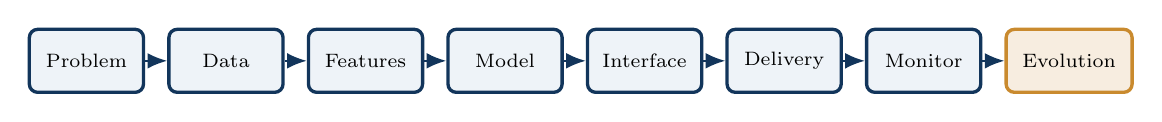
\begin{tikzpicture}[node distance=0.28cm]
  \node[flowbox, minimum width=1.45cm, minimum height=0.8cm] (problem) {\scriptsize Problem};
  \node[flowbox, minimum width=1.45cm, minimum height=0.8cm, right=of problem] (data) {\scriptsize Data};
  \node[flowbox, minimum width=1.45cm, minimum height=0.8cm, right=of data] (features) {\scriptsize Features};
  \node[flowbox, minimum width=1.45cm, minimum height=0.8cm, right=of features] (model) {\scriptsize Model};
  \node[flowbox, minimum width=1.45cm, minimum height=0.8cm, right=of model] (interface) {\scriptsize Interface};
  \node[flowbox, minimum width=1.45cm, minimum height=0.8cm, right=of interface] (delivery) {\scriptsize Delivery};
  \node[flowbox, minimum width=1.45cm, minimum height=0.8cm, right=of delivery] (monitor) {\scriptsize Monitor};
  \node[accentbox, minimum width=1.6cm, minimum height=0.8cm, right=of monitor] (evolution) {\scriptsize Evolution};
  \foreach \a/\b in {problem/data,data/features,features/model,model/interface,interface/delivery,delivery/monitor,monitor/evolution} {
    \draw[arrow] (\a) -- (\b);
  }
  \end{tikzpicture}

  \vspace{0.5em}
  \begin{block}{Today in the course}
  \textbf{Focus:} #1

  \textbf{Bridge:} #2
  \end{block}

  \begin{columns}[T]
  \column{0.48\textwidth}
  \begin{block}{Fraud case}
  {\footnotesize #3}
  \end{block}
  \column{0.48\textwidth}
  \begin{block}{Pasteurization case}
  {\footnotesize #4}
  \end{block}
  \end{columns}

  \vspace{0.3em}
  {\footnotesize \textbf{Course thread:} #5}
  \coursefooter
  \end{frame}
}

\newcommand{\classclosingframe}[4]{
  \begin{frame}{From This Class to the Next}
  \begin{block}{What stays with us}
  #1
  \end{block}

  \begin{columns}[T]
  \column{0.48\textwidth}
  \begin{block}{Project use}
  {\footnotesize #2}
  \end{block}
  \column{0.48\textwidth}
  \begin{block}{Next connection}
  {\footnotesize #3}
  \end{block}
  \end{columns}

  \vspace{0.3em}
  {\footnotesize \textbf{Course thread:} #4}
  \coursefooter
  \end{frame}
}

\tikzset{
  flowbox/.style={
    rounded corners=3pt,
    draw=courseblue,
    fill=courseice,
    very thick,
    minimum width=2.2cm,
    minimum height=0.9cm,
    align=center,
    font=\small
  },
  accentbox/.style={
    rounded corners=3pt,
    draw=coursegold,
    fill=coursegold!15,
    very thick,
    minimum width=2.2cm,
    minimum height=0.9cm,
    align=center,
    font=\small
  },
  arrow/.style={
    -{Latex[length=2.5mm,width=2mm]},
    thick,
    draw=courseblue
  }
}


\title{Class 4: Feature Engineering and Data Representation}
\author{\coursename}
\date{}

\begin{document}

\frame{\titlepage \coursefooter}

\begin{frame}{Agenda}
\begin{itemize}
\item Why feature engineering often matters more than model complexity.
\item Cleaning, curation, selection, extraction, and construction.
\item Encoding and transforming categorical, numerical, temporal, and streaming data.
\item Reproducible feature pipelines and leakage prevention.
\item Repository examples from fraud detection and pasteurization monitoring.
\end{itemize}
\coursefooter
\end{frame}

\begin{frame}{Learning goals}
\learninggoals{
\begin{itemize}
\item Distinguish feature engineering subtasks clearly.
\item Choose suitable encodings and transformations for different variable types.
\item Recognize leakage and feature availability problems.
\item Explain why feature logic must be reproducible across training and serving.
\end{itemize}
}
\coursefooter
\end{frame}

\coursecontextframe
{Feature representation and reproducible preprocessing.}
{This class converts exploratory findings into stable model inputs and prepares the handoff from data analysis to modeling.}
{In the fraud case, feature work means encoding transaction behavior, preventing leakage, and keeping preprocessing consistent across training and inference.}
{In the pasteurization case, feature work includes rates of change, state-aware variables, and derived indicators such as dTdt for process monitoring.}
{After this point, the course can talk about model quality because the representation problem has been made explicit.}

\begin{frame}{Why features matter so much}
\begin{itemize}
\item Models only learn from the representation we give them.
\item Better features can simplify the modeling problem dramatically.
\item Bad features can hide leakage, inject bias, or fail at inference time.
\item Feature quality usually determines whether deployment is robust or fragile.
\end{itemize}
\coursefooter
\end{frame}

\begin{frame}{Five related but different tasks}
\begin{tabularx}{\textwidth}{>{\bfseries}l X}
Cleaning & Fix missingness, duplicates, invalid values, and basic errors. \\
Curation & Organize, document, and validate datasets for reuse. \\
Selection & Keep the most informative existing variables. \\
Extraction & Transform variables into a new lower-dimensional representation. \\
Construction & Build new features from domain logic, time, aggregation, or combinations. \\
\end{tabularx}
\coursefooter
\end{frame}

\begin{frame}{Richer examples than textbook toy cases}
\begin{itemize}
\item Fraud detection: rolling transaction count, deviation from recent spending, merchant risk history.
\item Maintenance or process monitoring: moving average, slope, rate of change, state duration.
\item E-commerce: time since last purchase, category diversity, and promotion exposure.
\item Healthcare scheduling: no-show history, appointment lead time, and clinic congestion.
\end{itemize}
\coursefooter
\end{frame}

\begin{frame}{Encoding and transformation choices}
\begin{tabularx}{\textwidth}{>{\bfseries}l X}
One-hot encoding & Good for low-cardinality categories. \\
Ordinal encoding & Use only when order is real and meaningful. \\
Target encoding & Useful for high-cardinality categories, but must control leakage. \\
Scaling & Important for PCA, distance-based methods, and gradient-based models. \\
Cyclic encoding & Useful for hour-of-day, day-of-week, and seasonal variables. \\
\end{tabularx}
\coursefooter
\end{frame}

\begin{frame}[fragile]{Notebook example: missing values and typed filling}
\begin{lstlisting}[style=coursepython]
titanic = titanic.dropna(subset=["survived"])

for col in ["deck", "embark_town"]:
    titanic[col] = titanic[col].astype("category")
    titanic[col] = titanic[col].cat.add_categories("Unknown")
    titanic[col] = titanic[col].fillna("Unknown")

titanic["age"] = titanic["age"].fillna(titanic["age"].median())
titanic["embarked"] = titanic["embarked"].fillna("S")
\end{lstlisting}
\begin{itemize}
\item This follows `notebooks/Class4_DataEngineering.ipynb`.
\item The main lesson is that missing-value policy depends on column meaning, not on a single global rule.
\end{itemize}
\coursefooter
\end{frame}

\begin{frame}{Notebook plot: correlation before feature decisions}
\centering
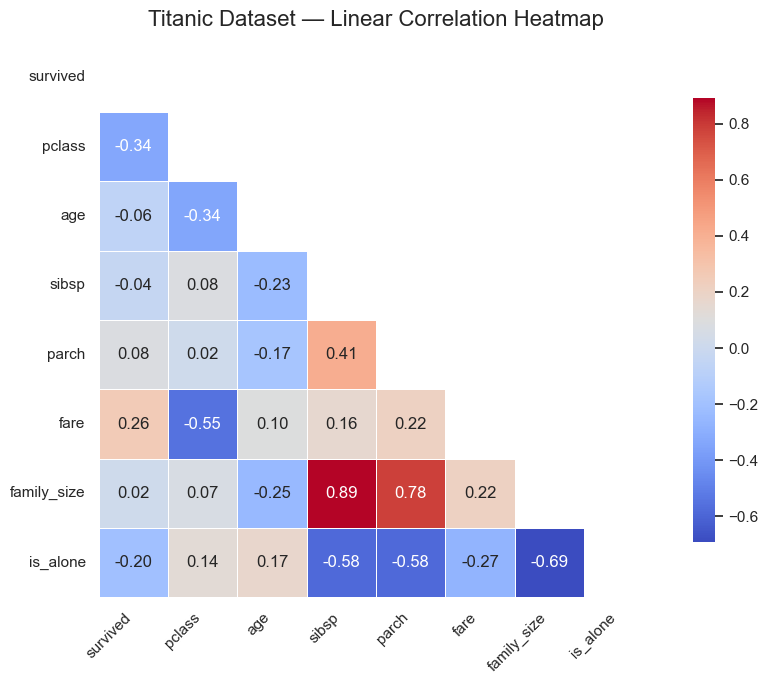
\includegraphics[height=0.74\textheight]{images/class04_titanic_correlation_heatmap.png}

{\scriptsize From `Class4_DataEngineering.ipynb`: a first pass at linear relationships in the Titanic variables before selection and construction.}
\coursefooter
\end{frame}

\begin{frame}[fragile]{Notebook example: constructing useful features}
\begin{lstlisting}[style=coursepython]
titanic["family_size"] = titanic["sibsp"] + titanic["parch"] + 1
titanic["is_alone"] = (titanic["family_size"] == 1).astype(int)
titanic["title"] = titanic["who"].map(
    {"man": "Mr", "woman": "Mrs", "child": "Master"}
)
\end{lstlisting}
\begin{itemize}
\item These are better examples than generic polynomial features because they reflect simple domain logic.
\item Students can discuss which features are causal hints, proxies, or redundant transformations.
\end{itemize}
\coursefooter
\end{frame}

\begin{frame}{Notebook plot: engineered features change the picture}
\centering
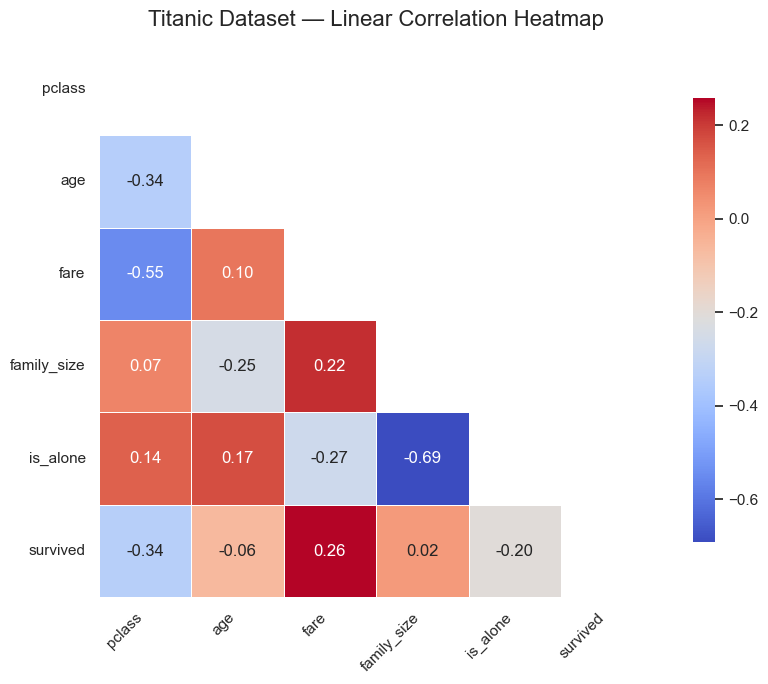
\includegraphics[height=0.74\textheight]{images/class04_engineered_feature_heatmap.png}

{\scriptsize The second heatmap from the notebook makes the new variables visible in relation to the target and the original numeric fields.}
\coursefooter
\end{frame}

\begin{frame}{Feature engineering for streams and sensors}
\begin{itemize}
\item Instantaneous values are often less informative than trends and rates.
\item Window-based features such as rolling means can reveal process stability.
\item State-aware features can distinguish normal variation from anomalies.
\item Streaming systems must compute features online, not only offline.
\end{itemize}
\begin{block}{Repository example}
`pasteurization/synth_sensors.py` already includes the derived feature `dTdt`, which is a simple but meaningful process feature.
\end{block}
\coursefooter
\end{frame}

\begin{frame}{Stream example: from raw signal to derived feature}
\centering
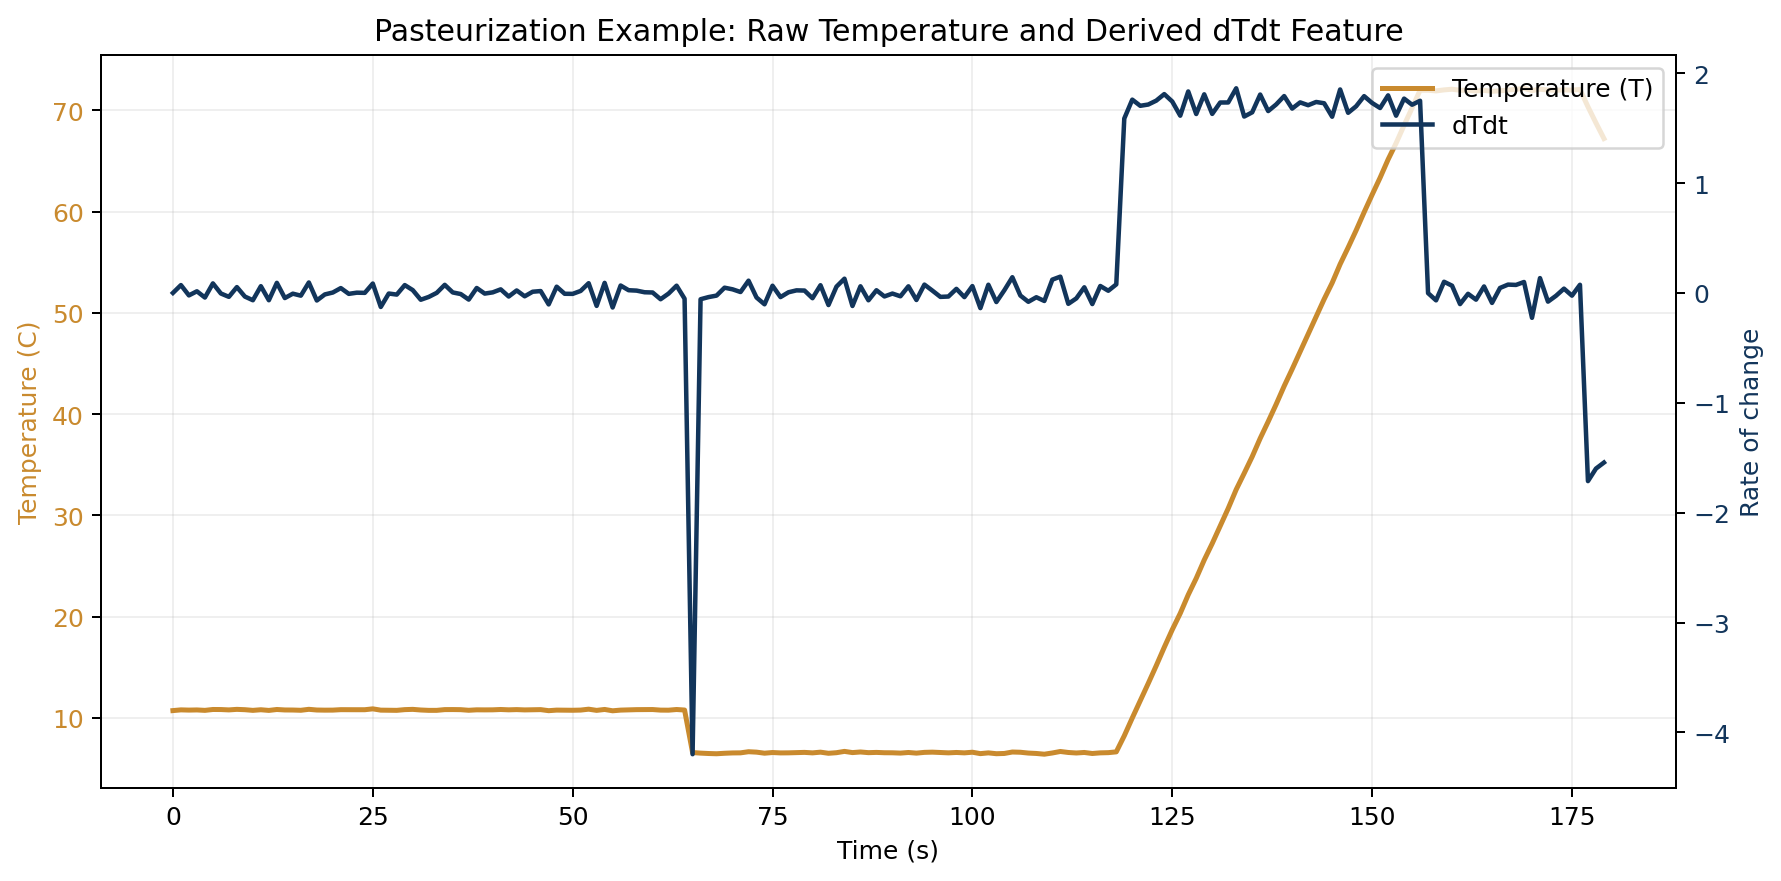
\includegraphics[height=0.72\textheight]{images/class04_pasteurization_dt_plot.png}

{\scriptsize In `pasteurization/synth_sensors.py`, `dTdt` is engineered from temperature to expose heating and cooling behavior more clearly than raw values alone.}
\coursefooter
\end{frame}

\begin{frame}{Feature pipelines in this repository}
\repoactivity{
\begin{itemize}
\item `notebooks/Class4_DataEngineering.ipynb` introduces tabular transformation logic.
\item `streamlit/modeling.py` and `streamlit/pages/App_Credit_Card.py` show why the scaler must be saved with the model.
\item `documents/FraudDetectionAsaService.pdf` describes a workflow where transformed variables ultimately feed an API.
\end{itemize}
}
\coursefooter
\end{frame}

\begin{frame}{Leakage and availability checks}
\begin{itemize}
\item Was the feature available at prediction time?
\item Does it encode future information, post-decision outcomes, or manual review results?
\item Will the feature be computed the same way in production?
\item Does the feature depend on unstable joins or missing upstream systems?
\end{itemize}
\coursefooter
\end{frame}

\begin{frame}{Why pipelines matter}
\begin{itemize}
\item Pipelines make preprocessing explicit and repeatable.
\item They reduce mismatch between training and inference.
\item They simplify testing, persistence, and model comparison.
\item They make handoffs between notebooks and services more reliable.
\end{itemize}
\coursefooter
\end{frame}

\begin{frame}{Notebook plot: chi-squared scores for categorical features}
\centering
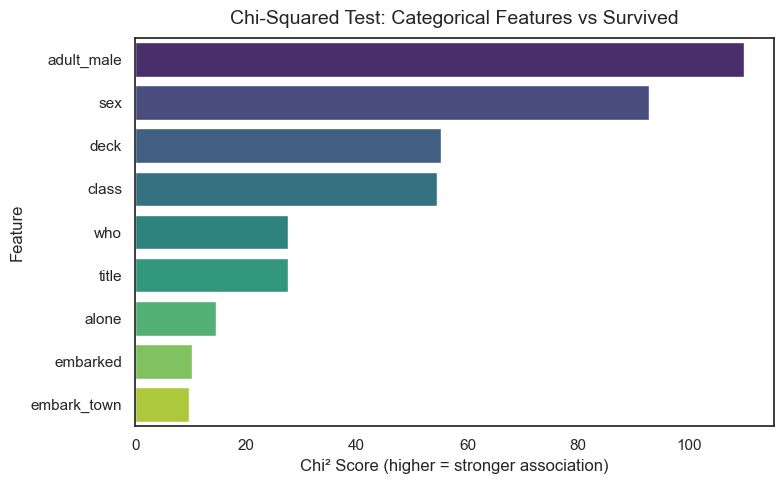
\includegraphics[height=0.72\textheight]{images/class04_chi2_feature_scores.png}

{\scriptsize This notebook figure helps explain selection: not every available categorical feature contributes equally to predicting the outcome.}
\coursefooter
\end{frame}

\begin{frame}[fragile]{Notebook example: preprocessing as a pipeline}
\begin{lstlisting}[style=coursepython]
numeric_features = ["age", "fare", "family_size"]
categorical_features = ["pclass", "sex", "embarked", "title"]

preprocessor = ColumnTransformer(
    transformers=[
        ("num", Pipeline([("scaler", StandardScaler())]), numeric_features),
        ("cat", Pipeline([("encoder", OneHotEncoder(handle_unknown="ignore"))]),
         categorical_features),
    ]
)
\end{lstlisting}
\begin{itemize}
\item This makes feature logic serializable, testable, and reusable in later modeling and serving stages.
\item It also reduces the chance of training-serving skew.
\end{itemize}
\coursefooter
\end{frame}

\begin{frame}{Technology links}
\readinglist{
\href{https://scikit-learn.org/stable/modules/compose.html}{scikit-learn pipelines and composite estimators};\ 
\href{https://scikit-learn.org/stable/modules/generated/sklearn.compose.ColumnTransformer.html}{ColumnTransformer};\ 
\href{https://pandas.pydata.org/docs/}{pandas documentation};\ 
\href{https://www.tensorflow.org/tfx/guide/transform}{TFX Transform}.
}
\coursefooter
\end{frame}

\classclosingframe
{\begin{itemize}
\item Features are engineered representations of domain assumptions, not raw columns passed through blindly.
\item Pipelines make preprocessing reproducible and reduce training-serving skew.
\item Better feature design can outperform more complex model choice.
\end{itemize}}
{Project teams should now be able to justify which variables to create, encode, scale, or discard and how that logic will stay consistent later.}
{Class 5 builds on these representations to compare models, metrics, baselines, and adaptation strategies.}
{Once features represent the problem well, the modeling step becomes a principled comparison instead of guesswork.}

\begin{frame}{Papers and materials}
\readinglist{
\href{https://www.oreilly.com/library/view/feature-engineering-for/9781491953235/}{Zheng and Casari, Feature Engineering for Machine Learning};\ 
\href{https://dl.acm.org/doi/10.1145/2347736.2347755}{Domingos (2012), A Few Useful Things to Know About Machine Learning};\ 
\href{https://www.jmlr.org/papers/volume12/pedregosa11a/pedregosa11a.pdf}{Pedregosa et al. (2011), scikit-learn};\ 
\href{https://www.tensorflow.org/tfx/guide/transform}{Reproducible preprocessing with TFX Transform}.
}
\coursefooter
\end{frame}

\end{document}
